\section{Прочие комбинаторные величины}

В этом параграфе мы очень кратко рассмотрим прочие комбинаторные величины, которые могут оказаться полезны и которые будут в дальнейшем выступать в качесве примеров.

\subsection{Числа Фибоначчи}

\begin{definition}
\term{Числа Фибоначчи} $F_n$ определяются начальными условиями $F_0 = 0$, $F_1 = 1$ и соотношением
$$F_{n+1} = F_n + F_{n-1}$$
\end{definition}

Начальные значения чисел Фибоначчи выглядят так:
$$0, 1, 1, 2, 3, 5, 8, 13, 21, 34, 55, \ldots$$

Эти числа возникают в целом ряде задач и довольно распространены. Исторически числа Фибоначчи стали широко известны после решения Леонардо Пизанским (<<Фибоначчи>>  было его прозвищем, что переводится как <<сын Боначчи>>) следующей задачи в 1202 году:

\begin{exercise}
Предположим, что каждая взрослая пара кроликов каждый месяц производит на свет ещё одну молодую пару кроликов. Взросление кроликов наступает в течение одного месяца. Изначально у нас есть одна пара молодых кроликов. Через месяц она становится взрослой. Еще через месяц эта пара производит на свет ещё пару молодых кроликов (итого 2 пары, из которых 1 молодая). В следующий месяц эта же пара производит ещё одну молодую пару, а пара, которая была молодой, взрослеет (имеем 3 пары кроликов, 1 молодая). Таким же образом в следующий месяц мы будем иметь 5 пар кроликов, из которых 2 будут молодыми. Сколько кроликов будет в конце года?
\end{exercise}

На самом деле числа, которые мы сегодня называем числами Фибоначчи, были известны ещё древним Индусам. Математик Пиндас в своём трактате <<Чхандас>> (датированным примерно 200 годом до нашей эры) использует их при решении примерно такой задачи:

\begin{exercise}
Пусть нам надо пройти путь длины $n$. При проходе пути мы можем использовать либо шаги длины 1, либо шаги длины 2. Докажите, что существует ровно $F_{n+1}$ способов пройти путь используя такие шаги. (Например, для пути длины 3 мы можем сделать три одинарных шага, либо вначале одинарный, а потом двойной, либо наоборот: итого 3 разных способа пройти путь).
\end{exercise}

Сами индусы, правда, решали хоть и ту же задачу, но из другой предметной области: они исследовали сколько всего существует мелодий, состоящих лишь из одной ноты, которая может иметь либо одинарную, либо двойную длительность. Интерпретация, данная привёденным мной упражнением, используется при решении следующих двух задач:

\begin{exercise}
Докажите следующее тождество, используя двойной счёт:
$$F_{n+1} = \sum_{k=0}^{\lfloor {n\over 2}\rfloor} {n-k\choose k}$$
\end{exercise}

\begin{exercise}
Докажите следующее тождество (идея доказательства очень похожа):
$$F_{n+1} = 1+ \sum_{k=0}^{n-1}F_n$$
\end{exercise}

\begin{thm}
$$F_n F_{n+1} = \sum_{i=1}^n F_i^2$$
\end{thm}
\begin{figure}[h]
\centering
\begin{tikzpicture}
\draw (0, 0) rectangle (6.5cm, -4cm);
\draw (2.5cm, 0) -- (2.5cm, -4cm);
\draw (0, -1.5cm) -- (2.5cm, -1.5cm);
\draw (1cm, 0) -- (1cm, -1.5cm);
\draw (0, -.5cm) -- (1cm, -.5cm);
\draw (.5cm, 0) -- (.5cm, -.5cm);
\end{tikzpicture}
\caption{Прямоугольник Фибоначчи}
\end{figure}
\begin{proof}
Идея доказательства продемонстрирована на рисунке~3.13. Прямоугольник Фибоначчи строится следующим образом: вначале рисуем квадрат с единичной длиной стороны. Затем справа от него рисуем ещё один такой же квадрат. После под ними рисуем квадрат со стороной равной двум предыдущим квадратам. Затем справа рисуем опять квадрат со стороной, равной двум предыдущим. Совершая последовательно $n$ таких построений, в итоге имеем прямоугольник со сторонами $F_n$ и $F_{n+1}$. Всего его площадь (то есть количество единичных квадратиков, которые в него уместятся), равно $F_nF_{n+1}$. В то же время подсчитав площади квадратов в порядке построения получаем сумму  $\sum_{i=1}^n F_i^2$.
\end{proof}

Следующая наша теорема (называемая теоремой Цекендорфа) утверждает, что любое натуральное число можно представить единственным образом в виде суммы чисел Фибоначчи таким образом, что каждое из чисел будет использоваться максимум единожды, и что в этой сумме не будут присутствовать никакие два последовательные числа Фибоначчи. Числа $F_1$ и $F_0$ в этом представлении так же не участвуют. Таким образом, для любого $a$ мы можем записать:
\begin{equation}\label{non:1}
a = \sum_{i=1}^m F_{\alpha_i}
\end{equation}
где $\alpha_k$~--- это последовательность номеров использованных чисел Фибоначчи.

Помимо интересного практического применения этой теоремы (о чём я напишу несколькими абзацами ниже), такое представление позволяет определить операцию <<фибоначчиевого умножения>>. Пусть, например, мы представили число $b$ так же в соответствии с теоремой Цекендорфа:
$$b = \sum_{j=1}^n F_{\beta_j}$$

Тогда умножение Фибоначчи определяется таким образом:
$$a\circ b = \sum_{i=1}^m\sum_{j=1}^n F_{\alpha_i+\beta_j}$$

\begin{exercise}
Покажите, что $2\circ3 = 13$ и что $4\circ4 = 40$.
\end{exercise}

Легко видеть, что такое умножение коммутативно ($a\circ b = b\circ a$), однако довольно неожиданно, что оно так же является и ассоциативным, то есть что выполняется тождество
$$a\circ(b\circ c) = (a\circ b)\circ c$$

Это в общем-то единственное полезное свойство такого умножения, но сам факт довольно интересен и неожиданнен. Доказательство, которое я представляю ниже, сделает это утверждение очевидным.

\begin{thm}
Любое число $n$ допускает единственное представление в виде \eqref{non:1}.
\end{thm}
\begin{proof}
Данная теорема может быть легко доказана по индукции (что и сделал в 1972 году Цекендорф), однако я представлю более остроумное доказательство, придуманное Дональном Кнутом в 1988 году. В той же работе Кнут ввёл понятие фибоначчиева умножения и показал его ассоциативность, как простое следствие из данного доказательства.

Теорему Цекендорфа можно переформулировать как возможность представить любое число в виде суммы
$$\sum_{i=0}^n d_iF_i$$
где коэффициенты $d_i$ могут принимать значения 0 или 1, причем два коэффициента подряд не могут принимать значение 1. Такую запись называют <<системой счисления Фибоначчи>>, поскольку она очень похожа на позиционные системы счисления, рассмотренные нами в~\S3.2, с той лишь разницей, что теперь вместо степеней некоторого основания мы используем значения $F_i$. По аналогии с позиционными системами счисления мы можем кратко записывать числа в ней, перечисляя последовательно коэффициенты $d_i$. Чтобы отличать фибоначчиеву систему счисления, мы будем подписывать букву $f$ справа от записи. Например,
$$33 = 101010100_f$$
Два младших разряда (соответствующие $F_0$ и $F_1$) всегда равны нулю.

Чтобы получить такую запись, мы вначале позволим коэффициентам $d_i$ принимать произвольные значения, а затем путём их преобразований будем пошагово идти к требуемому представлению. Заметим, что при отсутствии ограничений на коэффициенты, представить натуральное число $a$ в виде суммы чисел Фибоначчи не представляет труда: достаточно взять значения $d_2 = a$ и $d_i = 0$ в остальных случаях (или, иначе, можно применить тот же подход с остатками от деления, который мы применяли при построении позиционных систем счисления).

Пусть мы получили некоторую запись натурального числа в виде суммы чисел Фибоначчи без ограничений, и в ней имеется коэффициент $d_i > 1$. Здесь может быть две ситуации: когда $d_{i-1}> 0$ и когда $d_{i-1} = 0$. В первом случае мы можем увеличить на единицу значение $d_{i+1}$ и уменьшить на единицу значения $d_i$ и $d_{i-1}$. По определнию чисел Фибоначчи это не поменяет общую сумму. Замечу, что то же преобразование мы можем выполнить в случае
$$d_i = d_{i-1} = 1$$
Если же $d_{i-1} = 0$, то мы можем уменьшить на единицу $d_i$ и увеличить на единицу $d_{i-1}$ и $d_{i-2}$. Мы пришли к ситуации, когда $d_{i-1} > 0$, а как действовать в этом случае мы уже знаем. Применив указанное выше преобразование мы получаем суммарно, что мы увеличили на единицу $d_{i+1}$, уменьшили на двойку $d_i$ и на единицу $d_{i-2}$.

Если в ходе эти преобразований мы на каком-то шаге получаем $d_0 > 0$, то этот коэффициент можно безболезненно заменить на $d_0 = 0$. Если мы получили $d_1 > 0$, то можно смело прибавлять величину $d_1$ к $d_2$ зануляя $d_1$.

Здесь важно заметить два момента: во-первых, если рассматривать набор коэффициентов $\{d_i\}$ как упорядоченный набор, то после каждого такого преобразования новый набор будет больше старого в смысле лексикографического порядка. Применять одно из указанных преобразований мы можем всегда, если только наше число не представлено уже в требуемом виде. В то же время само множество допустимых наборов у нас ограничено, поскольку всегда найдётся $F_n > a$. Таким образом продолжать применять бесконечно долго наши правила преобразования мы не сможем. Отсюда следует, что в итоге мы обязательно придём к Фибоначчиевому представлению числа.

Из этой интерпретации легко увидеть и единственность такого представления. Если нам даны два различных представления числа, то мы можем вычесть меньшее в лексикографическом смысле из большего. Здесь правда может возникнуть проблема, что в каком-то разряде нам придётся вычитать единицу из нуля. Будем писать в этом случае $d_i =-1$, что означает, что этого слагаемого нам недостаёт. Поскольку мы вычитаем большее из меньшего, всегда найдётся такое $k$, что $d_{i+k} = 1$. Его можно занулить, увеличив на единицу значения $d_{i+k - 1}$ и $d_{i+k-2}$. Повторяя эту операцию несколько раз мы можем избавиться от всех значений $-1$, однако результат будет ненулевым, т.к. каждая такая операция не может уменьшать количество единиц в записи. Значит, разница между двумя представлениями будет ненулевой, а следовательно эти представления всё же задают различные числа.
\end{proof}

Очевидно теперь, что фибоначчиево умножение~--- это просто умножение чисел в столбик, с тем только лишь отличием, что мы на этот раз используем фибоначчиеву систему счисления. Отсюда уже легко понять, почему оно ассоциативно (поймите это в качестве упражнения).

В качестве приложения изложенного материала, рассмотрим задачу передачи данных по сети. Для просторы будем считать, что мы последовательно передаём числа в диапазоне от 0 до 15 (на практике мы вероятнее всего были бы заинтересованы в передаче полноценных байтов в диапазоне от 0 до 255). Кодировать числа мы будем битами 1 и 0, что означает наличие и отсутствие напряжения соответственно.

Конечно же, мы легко могли бы передать значения, используя простое двоичное представления. Пусть, например, мы хотим передать числа 11, 13 и 10. В двоичной записи мы передадим следующие данные:
$$1011\ 1101\ 1010\ \ldots \cong 11,13,10,\ldots$$
Однако, при передаче по сети данные могут теряться из-за помех. Пусть, например, мы потеряли четвёртый бит. Тогда полученные данные будут выглядеть как
$$1011\ 1011\ 0100\ \cong 11, 11, 4, \ldots$$
Очевидно, что все последующие данные так же будут повреждены и до получателя в результате дойдёт совершенно бессмысленный набор битов. Если, например, эти данные~--- видеотрансляция, то пропажа всего одного бита в потоке (что очень вероятно) по сути приведёт к неутсранимой ошибке, что заставит пользователя устанавливать соединение заново. Это явно неприемлемо, если вы хотите посмотреть видео через Интернет, или, скажем, сделать звонок в Нидерланды.

Трудность с двоичным представление возникает из-за того, что у нас нет никакого способа отделить один блок данных от другого. Фибоначчиева система счисления может решить проблему. Её критическим свойством является то, что в ней не могут идти подряд два бита 1, а значит мы можем использовать битовую последовательность 11 в качестве разделителя. Для экономии трафика (количества передаваемых данных) мы можем немного даже сэкономить, избавившись, во-первых, от разрядов $d_0$ и $d_1$ (они всегда нулевые), а так же передавая запись в обратном порядке. Это гарантирует нам, что старшим битом в записи всегда будет 1, поэтому мы можем дописывать всего один бит 1 к нему, а не биты 11. Например, если закодировать таким образом $11=1010000_f$, то в итоге получим значение $001011$, что короче на один бит. Данные, приведённые выше, будет таким образом переданы в виде
$$001011\ 0000011\ 010011\ \ldots \cong 11, 13, 10, \ldots$$
Если теперь у нас произойдёт ошибка связи и какой-то бит потеряется, вставится или изменится, мы конечно получим какие-то данные в ошибочном виде, однако мы всегда знаем, что новое значение начинается после последовательности 11, поэтому любое повреждение будет иметь лишь локальный характер. Опять же в случае видеопотока такое повреждение будет означать, что помеха отразится лишь на несколько кадров, однако эта помеха сама же и устранится, т.к. последующие данные мы будем получать уже в корректном виде.

На практике, впрочем, разработано множество других более совершенных систем кодирования, но их мы касаться не будем.

\subsection{Числа Каталана}

\begin{definition}
\term{Числа Каталана} $C_n$ определяются начальным значением $C_0 = 1$ и условием
$$C_{n+1} = \sum_{k=0}^n C_kC_{n-k}$$
\end{definition}

Начальные значения чисел Каталана выглядят так:
$$1, 1, 2, 5, 14, 42, 132, 429, 1430, 4862, 16796, \ldots$$

Как и числа Фибоначчи, они возникают во многих задачах. Рассмотрим, например, количество строк длин $n$, состоящих из парных скобок (то есть строк типа "((()()))(())"). Пусть у нас имеется $n+1$ парная скобка. Возьмём первую пару (то есть скобки "(...)..."). Предположим, что внутри этой пары находится $k$ пар скобок. Тогда после этой пары скобок будет находиться ещё $n-k$ пар скобок. По индукции это даёт нам, что всего таких строк есть $C_kC_{n-k}$ штук. Суммируя теперь по всем значениям $k$ получаем, что количество таких строк определяется числами Каталана.

Давайте теперь подсчитаем количество способов вычислить сумму (или любую другую ассоциативную операцию) $n+1$ слагаемых. В силу ассоциативности эта величина равна количеству способов расставить $n$ пар скобок в этой записи. Итого опять же получаем, что это количество способов вычислить сумму равно величине $C_n$.

По расстановке скобок в сумме мы можем построить бинарное дерево. Пусть у нас есть $n+1$ слагаемое. Вначале сопоставим каждому слагаемому в соответствие узел дерева (эти узлы будем называть \term{внешними}~--- они не будут имеют потомков). Затем каждой арифметической операции будем ставить в соответствие узел дерева с двумя потомками, соответствующими складываемым значениям (будем называть такие узлы \term{внутренними}). Очевидно, что такие деревья однозначно соответствуют расстановкам скобок, и следовательно таких деревьев будет $C_n$ штук. Здесь $n$~--- это количество операций, оно же количество внутренних узлов (внешних соответственно $n+1$). Если отбросить интерпретацию со слагаемыми, внешними и внутренними узлами, то получаем, что всего бинарных деревьев с $n$ узлами имеется $C_n$ штук. Рисунок~3.14 демонстрирует идею.

\begin{figure}[h]
\centering
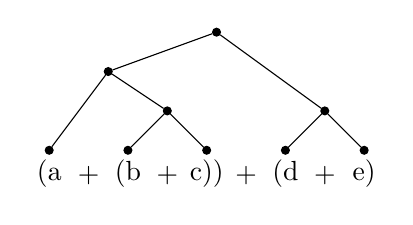
\begin{tikzpicture}
\def\point{node [circle, draw, fill, inner sep = 0, minimum size = .1cm] }
\def\emptynode{node [draw=none,fill=none, below] }
\draw (-2cm, 0) \point (p1) {};
\draw (-1.5cm, .05cm) \emptynode (s12) {};
\draw (-1cm, 0) \point (p2) {};
\draw (-.5cm, .05cm) \emptynode (s23) {};
\draw (0cm, 0) \point (p3) {};
\draw (.5cm, .05cm) \emptynode (s34) {};
\draw (1cm, 0) \point (p4) {};
\draw (1.5cm, .05cm) \emptynode (s45) {};
\draw (2cm, 0) \point (p5) {};

\draw (-.5cm, .5cm) \point (p23) {};
\draw (1.5cm, .5cm) \point (p45) {};
\draw (-1.25cm, 1cm) \point (p123) {};
\draw (.125cm, 1.5cm) \point (p12345) {};

\node [below] at (p1) {(a};
\node [below] at (s12) {+};
\node [below] at (p2) {(b};
\node [below] at (s23) {+};
\node [below] at (p3) {c))};
\node [below] at (s34) {+};
\node [below] at (p4) {(d};
\node [below] at (s45) {+};
\node [below] at (p5) {e)};

\draw (p23) -- (p2);
\draw (p23) -- (p3);
\draw (p45) -- (p4);
\draw (p45) -- (p5);
\draw (p123) -- (p1);
\draw (p123) -- (p23);
\draw (p12345) -- (p123);
\draw (p12345) -- (p45);
\end{tikzpicture}
\caption{Бинарное дерево, построенное по выражению.}
\end{figure}

Стоит отдельно заострить внимание на отличиях от тех деревьев, формулу для числа которых мы получили в теореме~3.42:
\begin{enumerate}
\item Дерево обладает корнем;
\item Вершины не имеют именований, важна только их форма;
\item Каждая вершина может иметь максимум двух потомков;
\item Рёбра упорядочены, то есть важно, нарисовано оно слева или справа от узла.
\end{enumerate}

На самом деле та же величина за небольшой оговоркой показывает и количество произвольных деревьев. Для того, чтобы увидеть это, нам потребуется следующее определение.

\begin{definition}
\term{Лесом} называется граф, состоящий из нескольких деревьев.
\end{definition}

Опять же леса рассматриваются в математике разные, но нас будут интересовать лишь те, в которых упорядочены как сами деревья, так и их рёбра. Оказывается, что между бинарными деревьями и лесами можно построить взаимооднозначное соответствие. Я покажу как по лесу построить бинарное дерево, процедура в обратную сторону совершенно аналогична.

В качестве корня бинарного дерева выбирается корень первого дерева в лесе. На рисунке 3.15 это узел $a$. Затем по левой ветви мы строим опять же бинарное дерево, которое строится по аналогии, если рассматривать первое дерево за вычетом корня, как лес (в примере на рисунке это лес, состоящий из деревьев d-h, e-i и f). По правой ветви мы строим бинарное дерево для леса, получающегося после удаления первого дерева (в примере это лес, состоящий из деревьев b-g и c). Имея бинарное дерево, мы можем восстановить по нему первоначальный лес, применяя те же операции в обратном порядке.

\begin{figure}[h]
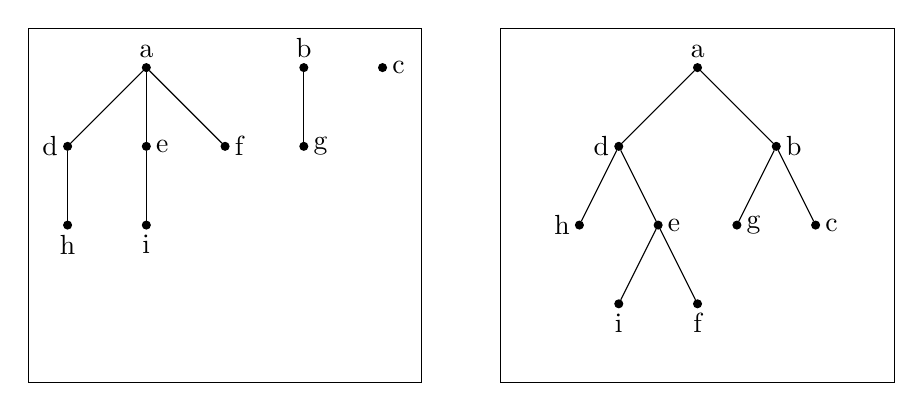
\begin{tikzpicture}
\def\point{node [circle, draw, fill, inner sep = 0, minimum size = .1cm] }
\draw (-1cm, 0) \point (lc) {};
\draw (-2cm, 0) \point (lb) {};
\draw (-2cm, -1cm) \point (lg) {};
\draw (-4cm, 0) \point (la) {};
\draw (-4cm, -1cm) \point (le) {};
\draw (-5cm, -1cm) \point (ld) {};
\draw (-3cm, -1cm) \point (lf) {};
\draw (-5cm, -2cm) \point (lh) {};
\draw (-4cm, -2cm) \point (li) {};

\node [right] at (lc) {c};
\node [above] at (lb) {b};
\node [right] at (lg) {g};
\node [above] at (la) {a};
\node [left] at (ld) {d};
\node [right] at (le) {e};
\node [right] at (lf) {f};
\node [below] at (lh) {h};
\node [below] at (li) {i};

\draw (lb) -- (lg);
\draw (la) -- (ld);
\draw (ld) -- (lh);
\draw (la) -- (le);
\draw (le) -- (li);
\draw (la) -- (lf);

\draw (-5.5cm, .5cm) rectangle (-.5cm, -4cm);


\draw (3cm, 0) \point (ra) {};
\draw (2cm, -1cm) \point (rd) {};
\draw (4cm, -1cm) \point (rb) {};
\draw (1.5cm, -2cm) \point (rh) {};
\draw (2.5cm, -2cm) \point (re) {};
\draw (3.5cm, -2cm) \point (rg) {};
\draw (4.5cm, -2cm) \point (rc) {};
\draw (2cm, -3cm) \point (ri) {};
\draw (3cm, -3cm) \point (rf) {};

\node [above] at (ra) {a};
\node [right] at (rb) {b};
\node [right] at (rc) {c};
\node [left] at (rd) {d};
\node [right] at (re) {e};
\node [below] at (rf) {f};
\node [right] at (rg) {g};
\node [left] at (rh) {h};
\node [below] at (ri) {i};

\draw (ra) -- (rd);
\draw (rd) -- (rh);
\draw (rd) -- (re);
\draw (re) -- (ri);
\draw (re) -- (rf);
\draw (ra) -- (rb);
\draw (rb) -- (rg);
\draw (rb) -- (rc);

\draw (5.5cm, .5cm) rectangle (.5cm, -4cm);
\end{tikzpicture}
\caption{Соответствие леса и бинарного дерева.}
\end{figure}

Теперь мы готовы к тому, чтобы понять сколько всего произвольных деревьев с $n$ вершинами существует. Если применить приведённую конструкцию к одному дереву, то полученное нами бинарное дерево не будет иметь правой ветви у корня, левое же его поддерево может быть произвольным бинарным. Итого у нас есть свобода выбора как расположить в дереве $n-1$ узлов. Всего произвольных деревьев с $n$ вершинами таким образом существует $C_{n-1}$ штук.

Ну и так далее, примеров можно привести ещё множество. Числа Каталана всплывают постоянно и мне даже кажется довольно странным, что они гораздо меньше известны в народе, нежели тех же числа Фибоначчи, которые зачем-то применяют даже биржевые трейдеры (последние верят, что числа Фибоначчи имеют какое-то психологически-сакральное значение, что позволяет им предсказывать поведение цен на рынке). Думаю, в пользе чисел Каталана я вас убедил. Остаётся вопрос о том как можно их более эффективно находить.

Числа Каталана можно интерпретировать ещё вот как. Рассмотрим квадрат размером $n\times n$. Положение в этом квадрата будем записывать парой $(x, y)$, которую будем называть \term{координатами}. $x$ и $y$ могут принимать значения от 0 до $n$. Мы начинаем движение из точки с координатами $(0, 0)$ и двигаемся в точку $(n, n)$, увеличивая за один шаг либо координату $x$, либо координату $y$ на единицу. Числа Каталана в этом случае показывают количество путей, которые не пересекают диагональ квадрата (то есть никогда не заходят в точку с координатами $(x, x+1)$).

Увидеть это довольно легко по индукции. Пусть утверждение уже доказано для квадратов размером вплоть до $n$ и мы рассматриваем количество путей в квадрате со сторонами $n+1$. Пусть при движении мы в последний раз касаемся диагонали в позиции $(k, k)$. Количество способов пройти такой путь до точки касания есть $C_k$ (по предположению индукции). После этого дойти до финиша не коснувшись диагонали у нас остаётся $С_{n-k}$ способов (пройти нам надо ещё $n-k+1$ клетку, однако учитывая, что мы не должны касаться диагонали, первый шаг у нас увеличит координату $x$, а последний координату $y$, что по сути сводит задачу к нахождению пути в квадрате со стороной $n-k$). Отсюда следует, что такие пути так же задаются числами Каталана.

С другой стороны те читатели которые читают учебник последовательно, помнят, что вообще-то ровно то же самое количество путей не пересекающих диагональ квадрата предлагалось найти в упражнении~3.60 используя только понятие сочетаний. Я покажу сейчас, как эта задача решается.

Вначале поймём сколько вообще существует путей, увеличивающих за шаг лишь одну координату, без учёта пересечения диагонали (упражнение~3.59). Если размеры прямоугольинка $m\times n$, то нам надо $m$ раз увеличить координату $x$ и $n$ раз координату $y$. Итого нам надо совершить $m+n$ шагов, из которых надо выбрать $m$ шагов, которые увеличивают $x$. Способов сделать такой выбор имеется ${m + n \choose m}$. В случае, если нам дан квадрат размером $n\times n$, то количество путей будет равно ${2n\choose n}$.

\begin{figure}[h]
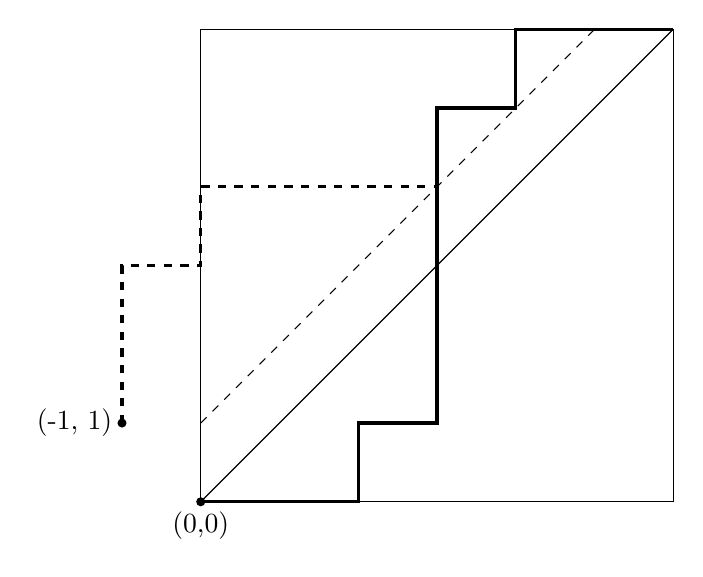
\begin{tikzpicture}
\def\point{node [circle, draw, fill, inner sep = 0, minimum size = .1cm] }
\centering
\draw (-3cm, -3cm) rectangle (3cm, 3cm);
\draw (-3cm, -3cm) \point (z) {};
\node [below] at (z) {(0,0)};

\draw (-3cm, -3cm) -- (3cm, 3cm);

\draw [very thick] (-3cm, -3cm) -- (-1cm, -3cm) -- (-1cm, -2cm) -- (0, -2cm) -- (0, 2cm) -- (1cm, 2cm) -- (1cm, 3cm) -- (3cm, 3cm);
\draw [dashed] (-3cm, -2cm) -- (2cm, 3cm);
\draw [very thick, dashed] (-4cm, -2cm) -- (-4cm, 0) -- (-3cm, 0) -- (-3cm, 1cm) -- (0, 1cm);

\draw (-4cm, -2cm) \point (t) {};
\node [left] at (t) {(-1, 1)};

\end{tikzpicture}
\caption{Отражение начала пути от диагонали.}
\end{figure}

Рассмотрим теперь путь, который диагональ всё же пересекает. Пусть после первого пересечения мы оказались в позиции $(k, k+1)$. Давайте отразим часть пути до этой точки относительно диагонали, сдвинутой вверх на единицу (см. рисунок 3.16). При этом получится некий путь, начинающийся в координатах $(-1, 1)$ и идущий в точку $(n, n)$. Таких путей ровно ${2n\choose n-1}$ штук, поскольку они описывают движение в прямоугольнике $((n-1)\times (n+1)$. Легко так же увидеть, что все пути из точки $(-1, 1)$ после отражения их от начала до точки пересечения диагонали (а они её пересекут обязательно) дают нам путь в начальном квадрате, который нас не устраивает, причём отношение это опять же взаимооднозначное. Итого нам осталось вычесть количество <<неправильных путей>> из общего числа путей:
$$C_n = {2n\choose n} - {2n\choose n-1} = {{2n\choose n}\over n+1}$$
Последнее равенство легко проверяется, я предлагаю вам выполнить проверку в качестве упражнения.

\subsection{Числа Рамсея}

Эта секция, вероятно, окажется наименее полезной и прикладной из всего, что до сих пор было в учебнике, однако сам результат, изложенный ниже, кого-то может удивить и даже показаться эстетически красивым. Лишним в любом случае не будет.

Напомню, что полным графом $K_n$ мы условились называть граф с $n$ вершинами такой, что любые две его вершины соединены рёбрами. Для нужд этого параграфа мы будем так же считать, что ребра графа разукрашены в разные цвета, которых всего имеется $m$ штук (это предположение эквиваленто заданию отображения $c:E\to[m]$, где $E$~--- множество ребер графа).

\begin{definition}
\term{Числом Рамсея} $r = R(c_1, c_2, \ldots, c_m)$ называется такая величина, что любой граф $K_n, n\ge r$ будет иметь хотя бы один подграф $K_{c_i}$, ребра которого целиком окрашены в цвет $i$.
\end{definition}

Пока это определение наверняка выглядит слишком абстрактно и непонятно. Давайте для примера рассмотрим число Рамсея $R(3, 3)$. Здесь речь идёт о раскраске графа в два цвета (назовём их для определённости синим и красным) и число $R(3, 3)$ показывает минимальное количество вершин, которое должен иметь полный граф, чтобы в нём обязательно нашёлся либо красный подграф $K_3$, либо синий подграф $K_3$. (Обратите внимание, что сам граф $K_3$ имеет вид треугольника).

\begin{exercise}
Раскрасьте в два цвета рёбра графа $K_5$ таким образом, чтобы в нём не было одноцветного треугольника.
\end{exercise}

Из приведённого упражнения следует, что $R(3,3)>5$. Давайте теперь рассмотрим граф $K_6$. Возьмём некоторую его вершину $a$. Из этой вершины исходит пять рёбер и среди них обязательно должно быть по крайней мере три ребра одного цвета. Для определённости будем считать, что это три красных ребра, ведущих в вершины $x$, $y$ и $z$. Если так сложилось, что все три ребра, соединяющие $xyz$ синие, то мы получили синий треугольник $K_3$. Если же среди этих ребёр найдётся красный (пусть, для определённости, это ребро $xy$), то мы имеем красный треугольник $axy$. Таким образом мы в любом случае будем иметь либо синий $K_3$-подграф, либо красный, и, следовательно, $R(3, 3) = 6$.

Приведённые рассуждения часто формулируют в виде следующей задачи: докажите, что среди группы из шести произвольных людей либо найдутся трое попарно знакомых друг с другом, либо трое попарно не знакомых. Эта задача требует по сути доказать, что $R(3, 3) \le 6$, если обозначить людей за вершины графа, а ребра раскрасить в соответствии с тем, знакомы эти люди или нет.

Что совершенно неочевидно про числа Рамсея, так это то что они вообще в принципе существуют. Пусть мы раскрашиваем граф в три цвета: красный, желтый и зеленый. Верно ли, что любой достаточно большой граф $K_n$ всегда будет иметь либо красный $K_{12}$-подграф, либо зелёный $K_{351}$-подграф, либо жёлтый $K_{12422}$-подграф? То что любой довольно большой граф удовлетворяет этому свойству само по себе удивительно и до предъявления строгого доказательства должно вызывать сомнения. Однако это так.

Мы разобьём доказательство того, что числа Рамсея всегда определы, на два этапа. Вначале мы докажем, что числа Рамсея определены для двухцветных раскрасок, а затем перейдём к общему случаю.

\begin{thm}
Число Рамсея $R(a, b)$ всегда определено, и, более того,
$$R(a, b) \le R(a - 1, b) + R(a, b- 1)$$
\end{thm}
\begin{proof}
Если мы докажем неравенство, то утверждение о существовании чисел Рамсея будет следовать из него само собой. Поэтому сразу возьмёмся за неравенство. Предположим по индукции, что оно выполняется для всех значений $R(x, y)$, где по крайней мере либо $x<a$ либо $y<b$. Первый цвет будем называть красным, второй синим. Рассмотрим полный граф с
$$R(a - 1, b) + R(a, b- 1)$$
вершинами и возьмём в нём произвольную вершину $x$. Опять же по обобщённому принципу Дирихле с ним инцидентно либо $R(a-1, b)$ красных рёбер, либо $R(a, b-1)$ синих. Пусть верно первое (второй случай рассматривается аналогично). Рассмотрим все вершины, соединённые с $x$ красными рёбрами. Эти вершины образуют подграф $K_{R(a-1, b)}$. По предположению индукции он либо имеет красный $K_{a-1}$-подграф, либо синий $K_b$-подграф. В последнем случае требуемый подграф найден, в первом же случае мы можем добавить к красному графу $K_{a-1}$ вершину $x$, и, поскольку она соединена с вершинами $K_{R(a-1, b)}$ красными ребрами, мы получаем красный $K_a$-подграф.
\end{proof}

\begin{exercise}
Докажите, что
$$R(a, b) \le {a+b-2\choose a - 1}$$
\end{exercise}

\begin{thm}
Число Рамсея $R(c_1, c_2, \ldots, c_m)$ всегда определено, и, более того,
$$R(c_1, \ldots,c_{m-2}, c_{m-1}, c_m) \le R(c_1, \ldots, c_{m-2}, R(c_{m-1}, c_m)$$
\end{thm}
\begin{proof}
Опять же существование числа Рамсея следует из неравенства. Доказывать мы его будем опять по индукции, но на этот раз будем проводить её по количеству цветов. Предположим, что для количества цветов, меньшего $m$, утверждение верно. Далее, забудем на некоторое время различие между цветами $m-1$ и $m$ и будем считать их эквивалентными. Если взять полный граф с
$$R(c_1, \ldots, c_{m-2}, R(c_{m-1}, c_m))$$
вершинами, то он будет либо иметь $K_{c_i}$-подграф цвета $i$, если $i<m-1$, либо же будет иметь $K_{R(c_{m-1}, c_m)}$-подграф с рёбрами цветов $m-1$ и $m$. В первом случае требуемое доказано. В последнем случае по предположению индукции мы имеем внутри этого подграфа либо $K_{c_{m-1}}$-подграф цвета $m-1$, либо $K_{c_m}$-подграф цвета $m$.
\end{proof}

В отличии от всех предыдущих величин, которые мы приводили, числа Рамсея совершенно не поддаются вычислению (теоретически они могут быть вычислены, но сложность этого просто чудовищная). Например, до сих пор неизвестно значение $R(5, 5)$. Оценка, приведённая нами в упражнении~3.86 говорит нам о том, что $R(5, 5)\le70$. На самом деле в 1992 году было доказано\footnote{<<A new upper bound for the Ramsey number R (5, 5)>>, B.~McKay, S.~Radziszowski, 1992}, что $R(5, 5)\le 49$. Так же в 1987 было доказано, что $R(5, 5) > 42$. То есть всего у нас есть 7 вариантов чему оно может быть равно. Давайте посмотрим как можно было бы точно определить используя эту оценку число Рамсея.

Возьмём граф $K_{46}$~--- число 46 лежит посередине между двумя допустимыми границами, и в случае если мы подтвердим или опровергнем наличие раскрасок, не имеющих $K_5$-одноцветных подграфов, то мы сразу же улучшим существующий научный результат аж в два раза. Очевидный способ, как это можно проверить, это перебрать все возможные графы $K_{46}$. Он имеет $46\times45 = 2070$ ребёр, каждое из которых мы можем раскрасить в один из двух цветов. Итого мы имеем $2^{2070}$ различных раскрасок графов $K_{46}$. Чему равно $2^{2070}$ сказать очень сложно, но это очень много. Калькулятор не имеет столько цифр. Чтобы оценить масштаб этого числа, попробуйте просто подсчитать разные степени числа 2.

Не смотря на то что числа Рамсея практически невычислимы, сам факт их существования может иметь следствия. Пусть у нас есть некоторая последовательность (конечная или бесконечная). Если выкинуть из неё часть членов, то то что останется мы будем называть \term{подпоследовательностью}. Теория Рамсея даёт нам следующий результат:

\begin{exercise}
Докажите, используя теорему Рамсея, что для любых чисел $a$ и $b$ найдётся такое $n$, что любая последовательность длины $n$ различных чисел  будет иметь либо возрастающую подпоследовательность длины $a$, либо убывающую подпоследовательность длины $b$.
\end{exercise}

\begin{exercise}
На самом деле если не использовать теорию Рамсея, то прошлое утверждение можно уточнить. Докажите, используя принцип Дирихле и двойной счёт, что на самом деле любая последовательность длины $(a-1)(b-1)+1$ будет удовлетворять условиям прошлого упражнения. Для доказательства можно сопоставить каждому элементу последовательности $z_k$ пару $(x_k, y_k)$, где $x_k$~--- наибольшая длина возрастающей подпоследовательности, оканчивающийся в позиции $k$, а $y_k$~--- наибольшая длина убывающей подпоследовательности, оканчивающейся в позиции $k$. Данная уточнённая оценка называется \term{теоремой Эрдёша-Секереша}.
\end{exercise}

\begin{thm}
Для любого $r$ найдётся такое $n$, что как бы мы ни разбивали множество $[n]$ на $r$ частей, в одной из них всегда найдутся такие числа $x, y, z$ (не обязательно различные), что $x+y=z$.
\end{thm}
\begin{proof}
Раскрасим элементы множества $[n]$ в $r$ цветов. Построим граф $K_n$, раскрасив каждое ребро $xy, x>y$ тем цветом, в который было раскрашено число $x-y$. Из существования числа $R(3, \ldots, 3)$ следует, что если $n$ достаточно велико, то в $K_n$ найдётся треугольник, раскрашенный одним цветом. Это в свою очередь означает, что найдутся вершины $i> j> k$ такие, что числа $x=i-j$, $y=j-k$, $z=i-k$ раскрашены в один цвет. Очевидно, что $x + y = z$.
\end{proof}

Приведённая теорема называется теоремой Шура. Похожее решение имеют следующие два упражнения.

\begin{exercise}
Докажите, что для любого $r$ найдётся такое $n$, что при любом разбиении $[n]$ найдётся такой элемент разбиения, что в нём будут содержаться числа $a$, $b$, $a+b$, $c$, $b+c$, d, что для них выполняется соотношение
$$a+b+c = d$$
\end{exercise}

\begin{exercise}
Докажите, что теорема Шура останется верна, если наложить условие $x\not= y$.
\end{exercise}